\draftpagebreak
\section{Reuse Requirements and Design Implications}
\label{sec:implications}
\subsection{Critical Reuse Across Configurations}
\outline{Use Fig.~\ref{fig:critical-reuse} to show that typical full-load thresholds span about 1.6 to 38,867 input vectors, then develop one concrete crossing: at the illustrative reuse $U=128$, STT-MRAM is resident-bound in the short and typical scenarios (about 181 and 133), but streaming-bound in the long scenario (about 95). Connect the native threshold to Qwen3.5-2B and MiMo-V2.5-Pro QKV stages using the existing sequential full-tile service reference, for which both sides accumulate the same tile count. Keep this mapping as a component-service bound, with output reduction and other system costs outside its scope.}

For native $128\times128$ tiles, let $m_K=D/128$, $m_N=N_{\mathrm{proj}}/128$, and $M=m_Km_N$:
\begin{align}
 T_{S,\mathrm{comp}}&=MU\Delta_S,&
 T_{R,\mathrm{comp}}&=MT_R,\label{eq:tile-times}\\
 \rho_{\mathrm{eff}}&=\rho/m_N,&
 \tau_{\mathrm{eff}}&=\tau,\label{eq:effective-capacity}\\
 \SI^*_{\mathrm{eff}}&=\frac{\SI^*}{m_N}=\frac{U^*}{N_{\mathrm{proj}}}.
 \label{eq:effective-ridge}
\end{align}
The factor $M$ cancels at service balance. This reference uses one engine, full tiles without padding, and equal $U$ per tile; input replay is included in $T_{S,\mathrm{comp}}$.
\draftreserve{0.65in}{Explain the threshold span and one scenario crossing.}
\draftcolumnbreak
\begin{paperfigure}
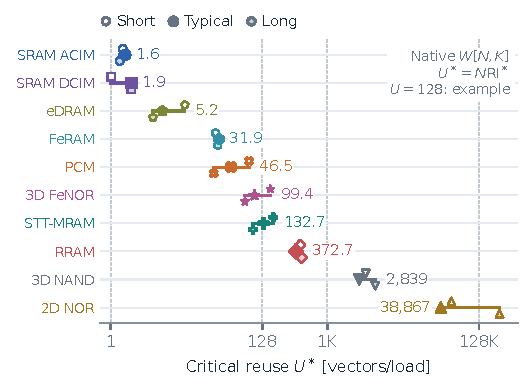
\includegraphics[width=\columnwidth]{figures/critical_reuse_single.pdf}
\caption{Full-load critical reuse $U^*=T_R/\Delta_S=N\SI^*$ at equal byte widths; each row uses its native $W[N,K]$. Numbers give typical values; segments span only three paired scenarios. Dashed lines mark illustrative reuse counts, not universal balance points. $1\Kilo=1024$.}
\label{fig:critical-reuse}
\end{paperfigure}

\subsection{Design Implications}
\outline{Turn a target reuse count into an allowable full-load service time using \eqref{eq:load-budget}, making Fig.~\ref{fig:critical-reuse} a design requirement rather than a ranking. Revisit Fig.~\ref{fig:hardware-capacities} to explain why a lower threshold alone does not imply higher performance: streaming throughput still sets the upper plateau. Contrast weight residency with growing attention state in Table~\ref{tab:workload-intensity}; KV append requires its own update-service boundary before applying any full-load threshold.}
\begin{equation}
  T_R\leq U_{\mathrm{target}}\Delta_S
  \quad\Longleftrightarrow\quad U_{\mathrm{target}}\geq U^*.
  \label{eq:load-budget}
\end{equation}
This is a necessary service-balance condition for reaching the streaming ceiling, not a guarantee of realized throughput.
\draftreserve{0.75in}{Turn a target reuse count into a resident-service requirement.}
